\documentclass{jlreq}
\usepackage[bookmarks=true,bookmarksnumbered=true,
pdftitle={Cracking the System Design Interview},
pdfauthor={nryotaro},
pdfkeywords={System Design; Interview},
pdflang=ja-JP]{hyperref}
\usepackage{graphicx}
\usepackage{main}
\addbibresource{main.bib}
\begin{document}
\title{Cracking the System Design Interview}
\author{nryotaro}
\date{\today}
\maketitle
\tableofcontents
\part{基本}
\begin{section-bib}{面接の流れ}
  システム全体のアーキテクチャを問われるときは、Propose a Design, Talk about trade-offs, Discuss design choices, Limitationsの4部構成で話す\cite{lc-high}。
\end{section-bib}
% 
\begin{section-bib}{モノリスではなくマイクロサービスで設計する}
  % モノリスとマイクロサービスの比較を書く。
  課題はモノリスで設計するには複雑すぎるので、マイクロサービスの設計を提案する\cite{lc-aa}。
  \subsection{設問}
  \begin{exercise}
  \item モノリスと比べたときのマイクロサービスの利点と欠点をのべよ。\label{exe:monolith-micro}  
  \end{exercise}
  \subsection{解説}
  \subsubsection*{\ref{exe:monolith-micro}}
  たとえば、複数の技術を適材適所に使えるが、プロセス内の通信がネットワーク越しのAPI呼び出しになる分のレイテンシーが発生する\cite{lc-aa}。  
\end{section-bib}

\begin{section-bib}{非同期メッセージング}
  ConsumerからProducerにキューを介してメッセージを送ることがある\cite{microsoft-messaging}。
  Producerでの失敗を伝えるために使えそう。
  また、メッセージのスパイクが起きてもブローカーがバッファとなり、負荷を平準化できる。
  \subsection{Queue}
  複数のサービスへ同期的に通信するトランザクションは、通信を非同期にすれば応答の待機時間を短くできる。
  しかし、対向サービスに障害があれば非同期通信が失敗しても、トランザクションは別のサービスにリクエストを送る。
  サービスをキューを介して通信させることで、対向サービスと一時的につながらない間でも、キューにメッセージを蓄積でき、メッセージの消失を防ぐことができる\cite{lc-isc}。
  \subsection{設問}
  \begin{exercise}
  \item 2つのサービスが直接ではなくキューを介して非同期通信する利点をのべよ。また、利点を満足するためのキューへの要件は何か。\label{exe:async-queue}
  \item 主要なメッセージキューのミドルウェアを挙げ、向き、不向きを比較せよ。\label{exe:queue-compare}
  \end{exercise}
  \subsection{解説}
  \subsubsection*{\ref{exe:async-queue}}
  対向システムの障害時のリクエストをキューに一時的に保存できるため、失敗するリクエストを減らすことができる\cite{lc-isc}。
  キューは、中継対象のシステムより、安定していなけばならない。
  キューでなくロードバランサでも負荷分散を実現できるので、キューの利点として負荷分散を先にあげるのはよくないだろうか。
  \subsubsection*{\ref{exe:queue-compare}}
  Kafka, RabbitMQ, ActiveMQがある\cite{lc-isc}。
\end{section-bib}
\begin{section-bib}{双方向通信}
  ロングポーリングは、タイムアウトまでの時間を長くし、サーバからの応答を待つ。
  このとき、サーバーはクライアウントのタイムアウトを検知できない\cite{sdi}。
  サーバーからの通知が必要でクライアントからの通知がいらなければ、WebSocketではなくEvent Sourceを使えるか検討するとよいかもしれない。
  2022年8月におけるTwitterのタイムラインには、Event Sourceが使われている。
  \subsection{設問}
  \begin{exercise}
  \item ロングポーリングとWebSocketそれぞれの使いどころを述べよ。
  \item WebsocketとEvent Sourceの利点欠点を比較せよ。
  \end{exercise}
\end{section-bib}
\begin{section-bib}{Pub/Sub}
  \subsection{Redis}
  RedisにはPub/Subの機能もある\cite{redis-pubsub}。
  ドキュメントを読む限り、すべてのSubscriberにメッセージをブロードキャストし、Ackによる再処理はできないよう。
\end{section-bib}
\begin{section-bib}{CQRS}
  CQRSはデータをコマンドとクエリの両方のモデルで永続化する\cite{microsoft-cqrs}。
  CQRSでEvent Sourcingが必須なのは、コマンドの永続化層にデータを書き込むのとをクエリの永続化層への追加したデータの通知を、1つのトランザクションで行い整合性を保つ必要があるから\cite{j5ik2o-cqrs-event-sourcing}。
\end{section-bib}
\begin{section-bib}{キャッシュ}
  \subsection{Consistent Hashing}
  キャッシュを複数のノードに分散して保存するとき、ハッシュ関数をキーに適用し、値が格納されたノードを特定できる。
  このとき、参加するノードが変われば、キャッシュされたデータを再配置しなければならない。
  コンシステントハッシュ法は、円環上のハッシュ値とノードを配置したとき、ハッシュ値から時計回りに出発し最初に出会うノードに値を格納する\cite{sdi}。
  このとき、ノードを追加、削除した場合に変更が起きた箇所付近の弧のノードだけをリバランスすればよく、再配置すべきデータ量を減らすことができる。
  ノードの数が少ないと、再配置した結果、ノードごとのデータ量が偏るおそれがある。
  ノードの数がおおいほど、偏りを防げるため、1つのノードに対応する複数の仮想的なノードを円環上に配置することで、偏りを抑止できる。
  
  Consistent Hasingは、CDNのようなインタネット規模のキャッシュシステムで使われる一方で、データベースのパーティショニングではうまくいかない\cite{DBLP:journals/corr/LampingV14}。
  \subsection{Cache Eviction}
  Cache evictionの方式にはTTL、FIFO, LFU, LRU, LFRUなどがある\cite{lc-cache}。
  \subsection{設問}
  \begin{exercise}
  \item Redisを使うアプリケーションを構築し、Redisの基本的な機能に習熟せよ。
  \end{exercise}
\end{section-bib}
\begin{section-bib}{分散ファイルシステム}
  CDNを使えば、Amazon S3などの分散ファイルシステムに配置したデータを高速に配信できる\cite{lc-databases}。
\end{section-bib}

\begin{section-bib}{データベース}
  % NOSQLの代表例, document指向の使いどろこ、列指向のつかいどころを説明させる。
  ACIDのConsistency(一貫性)は、データに常に真でなければならない不変性があることである\cite{ddia}。
  属性が多いデータはドキュメント指向データベースが、クエリのパターンが少ないがデータ量が多いときは列指向データベースがよい\cite{lc-databases}。
  ドキュメント指向データベースの例にMongoDBやCouchbaseが、列指向データベースの例にCassandraやHBaseがある。
  \subsection{設問}
  \begin{exercise}
  \item ACIDの各アルファベットが示す特性について説明せよ。
  \item Cassandraを使うアプリケーションを構築し、その基本的な機能に習熟せよ。
  \end{exercise}  
\end{section-bib}
\begin{section-bib}{Rate Limiting}
  \subsection{Leaky Bucket}
  蓄えられる未処理のリクエスト数と一定時間に処理できるリスエスト数の2つパラメータでリクエストを制御する\cite{sdi}。
  蓄えられている未処理のリクエストから一定時間内の固定数のリクエストを処理する。
  蓄えられるリクエスト数を越えてリクエストが届く場合リクエストを破棄する。
  パラメタ数が少なくチューニングが簡単だが、蓄えられるリクエスト数が一杯になるまでは、一定時間に処理できる分量以上のリクエストを受けつけてしまう。
  \subsection{Fixed Window}
  一定時間のウィンドウ内に処理するリクエスト数の上限を決め、それを越えるリクエストを破棄する。
  2つのウィンドウをまたいだ時刻にリクエストが多く到着する場合、ウィンドウサイズを越えたリクエスト数がウィンドウサイズと同じ時間内に処理されるおそれがある。
  \subsection{Sliding Window}
  一定時間のウィンドウをスライドさせ、Fixed windowのウィンドウをまたいだ場合に上限以上のリクエストが処理される問題をふせぐ。
  Fixed Windowよりも制御に多く計算リソースが必要である。
  \subsection{設問}
  \begin{exercise}
  \item リクエストの上限を制御するためのアルゴリズムをいくつか挙げ、その特徴をのべよ。
  \end{exercise}
\end{section-bib}
\part{Case Studies}
\begin{section-bib}{Google Maps}
  \subsection{LeetCode}
  解答は、ユーザの位置を特定する機能とユーザに道案内を提示する機能に対して個別のアーキテクチャ図を提示する\cite{lc-googlemaps}。
  ユーザの位置情報からマップを更新する。
  Spark Streaming Serviceは、新しいストリーミングサービスに置き変わった\cite{spark-streaming}。
  以下の機能要件は、二点間を移動中に距離とETAを随時通知することであり、ユーザが明示的にリクエストを移動中に送るだけではない。
  Google Mapは地図をcanvas要素で描画する。
  \begin{quote}
    Find distance and ETA while travelling between 2 points.
  \end{quote}
  
  \subsubsection{User Location Information}
  \begin{description}[labelsep=10pt]
  \item[Websocket Handler] ゲートウェイの役割。スケールアウトする。
  \item[Websocket Manager] デバイスがどのWebsocket Handlerと通信しているかを記録する。
  \item[Location Service] ユーザの位置情報を管理する。
  \item[Map Update Service] 新しい道などの地理的な変化を通知する。
  \item[Traffic Update Service] 移動速度の変化を通知する。
  \item[Graph Processing Service] グラフを更新する。
  \end{description}
  \subsubsection{User Navigation Flow}
  \begin{description}[labelsep=10pt]
  \item[Area Search Service] 現在値を緯度経度に変換する。
  \item[Navigation Tracking Service] ユーザが移動中に道案内を通知する。
  \item[Maps Service] ユーザからの道案内のリクエストを受けつける。
  \item[Historical data service] 過去のETAを蓄積し、最新のETAを計算できないときに、代替としてETAを提供する。
  \item[Segments]
  \end{description}
  \subsubsection{自分の解答}
  \href{https://docs.google.com/drawings/d/1w_a6eJVLqFsHHtm0dchQxM1NNOsW16ENjF7n_MRv6OE/edit}{編集中}
  \begin{figure}[ht]
    \centering
    \includegraphics[keepaspectratio, scale=0.25]
    {build/googlemaps/leetcode.eps} 
    \caption{Googlemapsの答案}
    \label{fig:lc-googlemaps}
  \end{figure}
\end{section-bib}
\begin{section-bib}{Amazon System Design}
  \href{https://docs.google.com/drawings/d/156NaHO0stF_xJBGtAUzkLmhU2eIz2ZYGaySqlPKHCLY/edit}{編集中}。
  解答\cite{lc-amazon}の問題点と長所をいれて改修する。
  データの更新情報のフローがない。
  非同期結果整合性でよくとりこぼしがないほうがいいところはkafkaにしよう。
  \begin{figure}[ht]
    \centering
    \includegraphics[keepaspectratio, scale=0.25]
    {build/amazon/leetcode.eps}
    \caption{Amazonの答案}
    \label{fig:lc-amazon}
  \end{figure}
\end{section-bib}
\begin{section-bib}{Facebook System Design}
  \subsection{LeetCode}
  \subsubsection{答案}
  \href{https://docs.google.com/drawings/d/1Xe7tRV1plpmUM1GEbcm1Rr-Sl4nuBaOe9AlLlUXsHQw/edit}{編集中}。
  タイムラインに表示すべきPostのユーザを管理するために必要な抽象データ構造は、ユーザIDからユーザIDの集合を要素とするハッシュテーブルであるため、タイムラインの表示にグラフDBはいらない。
  BFFを使うとオーケストレーターパターン\cite{microsoft-choreography}になってしまうのだろうか。
  メッセージサービスを制御の反転につかえそう。
  タイムラインの要件が曖昧であれば、タイムラインの順序が厳密な時系列であるべきか聞いたほうがよさそう。
  Postはスパイクする可能性があり、また、高速に保存するため、処理の平準化のためにメッセージングサービスを間においた。
  TimelineとBFFはEventSourceで通信する。Timelineがstored postsを取得したら通知する。
  
  \begin{figure}[ht]
    \centering
    \includegraphics[keepaspectratio, scale=0.20]
    {build/facebook/leetcode.eps}
    \caption{Facebookの答案}
    \label{fig:lc-facebook}
  \end{figure}
  \subsubsection{Leetcodeの解答}
  Post Injestion Service\cite{lc-facebook}はPostの書き込みを、Post Serviceは読み込みを担当しているが、永続化層はコマンドとクエリに分かれておらず、CQRSではない\cite{microsoft-cqrs}。
  Kafkaは、ポーリングを避けてイベントをほかのサービスに通知するために使われているのだろうか。
  KafkaのConsumerが失敗した場合の処理を考慮していないのではないか。
  \subsection{設問}
  \begin{exercise}
  \item CDNにおいたファイルへのアクセスに認証をかける手段を実在のサービスをまじえて例示せよ。
  \item Kafkaのメッセージの順序は到着順か。
  \item Cassandraは集計関数があるか。たとえば、Likeの総数を誰がどのPostにLikeしたかを示すレコードから集計できるか。
  \end{exercise}
\end{section-bib}
\begin{section-bib}{Airbnb System Design}
  \subsection{LeetCode}
  文章ではなく動画で解説がなされてる\cite{lc-airbnb}。
  動画のある機能要件と非機能要件を列挙する。
  模範回答のアーキテクチャは他のLeetCodeの回答とおなじくKafkaを多用した非同期アーキテクチャだが、System Design Interviewはメッセージングサービスを使っていない\cite{sdi2}。
  LeetCodeの回答はKafkaを使った非同期アーキテクチャに偏向しているように思える。

  氏名やアドレスなどのユーザの予約以外の情報を保存する専用のサービスがない。予約していないユーザデータもBookingに保存するのだろうか。
  \begin{itemize}
  \item 機能要件
    \begin{itemize}
    \item Hotel
      \begin{itemize}
      \item Onboarding
      \item Updating
      \item Bookings
      \end{itemize}
    \item User
      \begin{itemize}
      \item Search
      \item Book
      \item Check Bookings
      \end{itemize}
    \end{itemize}
  \item 非機能要件
    \begin{itemize}
    \item Low latency
    \item High availability
    \item High consistency
    \item Scale
      \begin{itemize}
      \item 500K hotels
      \item 10M rooms
      \item 1000 rooms / hotel (max 7,500)
      \end{itemize}
    \end{itemize}
  \end{itemize}
  \subsubsection{答案}
  \href{https://docs.google.com/drawings/d/1oregVo4fx3HTBSgF3dMn4DQ3X_REdrHiq2u5p3FegcQ/edit}{編集中}
  \begin{figure}[ht]
    \centering
    \includegraphics[keepaspectratio, scale=0.5]
    {build/airbnb/leetcode.eps}
    \caption{Airbnbの答案}
    \label{fig:lc-airbnb}
  \end{figure} 
\end{section-bib}
\end{document}